\chapter{Evaluation}
\label{cha:evaluation}

This section uses the application described in chapter \ref{cha:solution_details} in order to simulate various demo scenarios. For each scenario both the simplistic approach of just using rigid bodies is compared to the approach proposed in this thesis. The general layout of the scenario is always the same. At the center of the simulated world there is a block modeled as a simple rigid body. To both sides of this block are fingers. In the naive approach these fingers are also simple rigid bodies. For the other approach both fingers are implemented using the combination of a rigid inner bone and a soft outer tissue.

The fingers are simulated in such a way that they apply a constant force both in the direction of the block as well as in the upward direction. These two forces combined are then able to lift up the block from the ground. For each scenario a couple of small variations are tested in order to better understand and compare the implications of both types of approaches. The results for each simulation are compared using the offset of the block. For each simulation step the offset of the block's center of mass to its starting position's center of mass is calculated. The three coordinates are then plotted in order to provide an easily understandable visualization of the simulation results. 

Each different scenario is explained and illustrated on the following pages. Additional for each scenario a short video demonstration can be found on the accompanying CD.

\clearpage

\paragraph{Scenario 1}
In this scenario the fingers are perfectly aligned numerically with the block. This means the faces of the fingers are exactly perpendicular to the faces of the block. The block is a small box standing upright, comparable to a can.

\begin{figure}[htb]
	\setcounter{subfigure}{0}
	\centering
	  \subfigure{
	      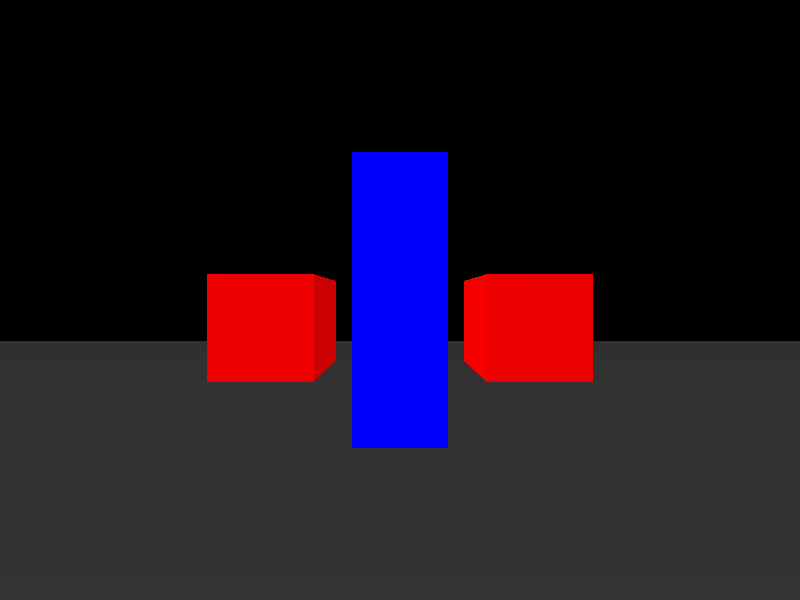
\includegraphics[width=.48\textwidth]{scenario1_rigid}
	  }
	  \subfigure{
	      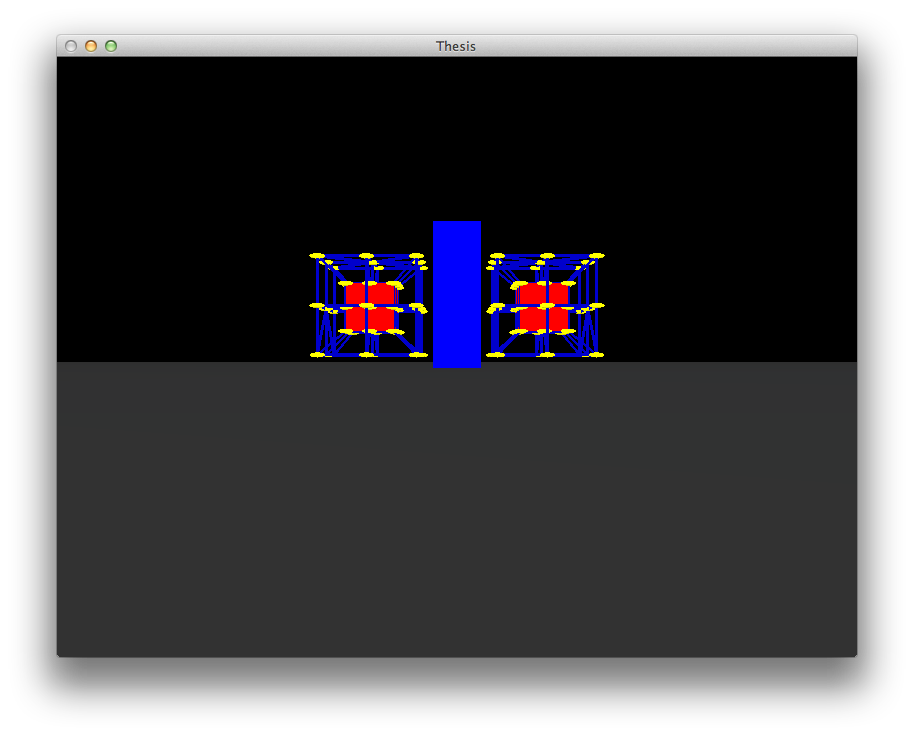
\includegraphics[width=.48\textwidth]{scenario1_combined}
	  }
	\setcounter{subfigure}{0}
	\subfigure[rigid fingers]{
		\begin{tikzpicture}
			\begin{axis}[xlabel=$time$,ylabel=$delta$,legend pos=north west]
				\addplot [color=red,mark=false,smooth,thick] table[x=time,y=err_x] {data/scenario1_rigid.txt};
				\addplot [color=green,mark=false,smooth,thick] table[x=time,y=err_y] {data/scenario1_rigid.txt};
				\addplot [color=blue,mark=false,smooth,thick] table[x=time,y=err_z] {data/scenario1_rigid.txt};
				\legend{$\Delta x$,$\Delta y$,$\Delta z$}
			\end{axis}
		\end{tikzpicture}
	}
	\subfigure[combined fingers]{
		\begin{tikzpicture}
			\begin{axis}[xlabel=$time$,ylabel=$delta$,legend pos=north west]
				\addplot [color=red,mark=false,smooth,thick] table[x=time,y=err_x] {data/scenario1_combined.txt};
				\addplot [color=green,mark=false,smooth,thick] table[x=time,y=err_y] {data/scenario1_combined.txt};
				\addplot [color=blue,mark=false,smooth,thick] table[x=time,y=err_z] {data/scenario1_combined.txt};
				\legend{$\Delta x$,$\Delta y$,$\Delta z$}
			\end{axis}
		\end{tikzpicture}
	}
	\caption{Evaluation Scenario 1}
\end{figure}

For this idealistic scenario the simple rigid body simulation still performs reasonably well. As expected from an analytical perspective $\Delta y$ is slowly accelerating upwards, while the block is slowly drifting in $\Delta z$, due to numerical instabilities. Eventually the block would fall out of the fingers The combined body simulation however has no issues holding onto the block also true for the combined body simulation which also performs as expected. The problem evident in the pure rigid body simulation is even more pronounced in the real world. Most of the time the mesh of the objects is a triangular mesh and the collisions cannot be resolved this cleanly. In addition the angles between the fingers and the object will almost never be perfectly perpendicular. In these more complex scenarios the simple rigid body simulation is expected to fail while the deformable body should continue to perform well.

\clearpage
\paragraph{Scenario 2}
The second scenario modifies the position of the fingers slightly. The fingers are now slightly rotated so they are not perfectly perpendicular anymore. Instead they are positioned more realistically like real fingers extending from the hand. This should make it harder for the rigid fingers to hold the block in center. The block itself remains unchanged to scenario 1.

\begin{figure}[htb]
	\setcounter{subfigure}{0}
	\centering
	  \subfigure{
	      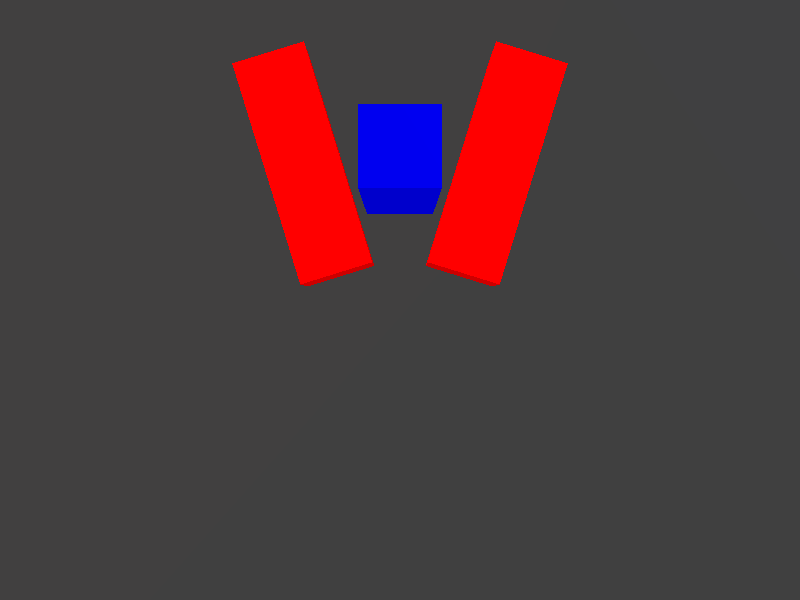
\includegraphics[width=.48\textwidth]{scenario2_rigid}
	  }
	  \subfigure{
	      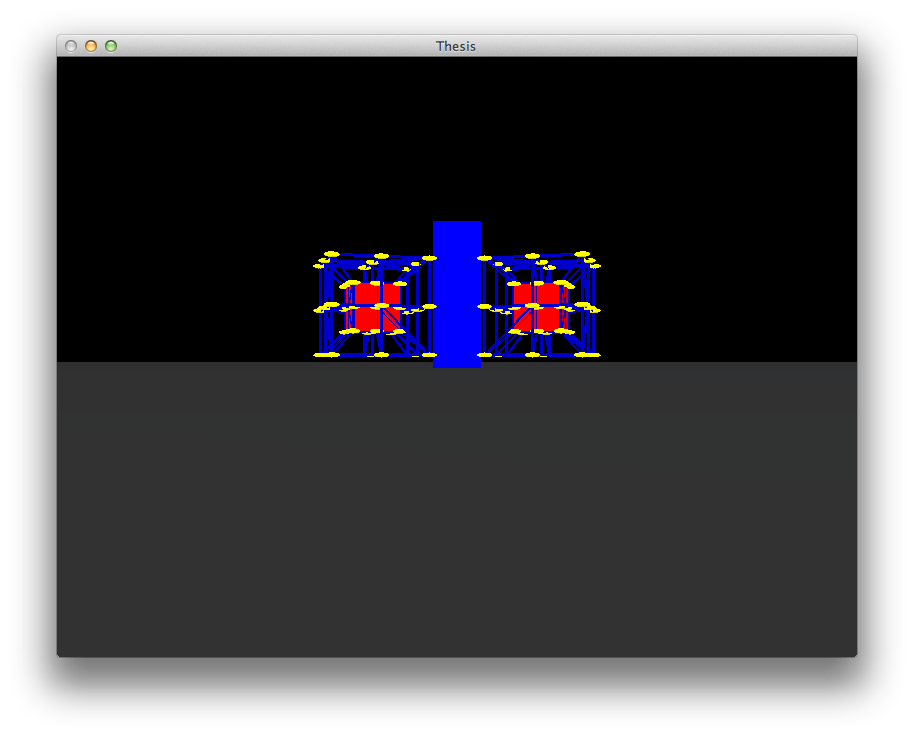
\includegraphics[width=.48\textwidth]{scenario2_combined}
	  }
	\setcounter{subfigure}{0}
	\subfigure[rigid fingers]{
		\begin{tikzpicture}
			\begin{axis}[xlabel=$time$,ylabel=$delta$]
				\addplot [color=red,mark=false,smooth,thick] table[x=time,y=err_x] {data/scenario2_rigid.txt};
				\addplot [color=green,mark=false,smooth,thick] table[x=time,y=err_y] {data/scenario2_rigid.txt};
				\addplot [color=blue,mark=false,smooth,thick] table[x=time,y=err_z] {data/scenario2_rigid.txt};
				\legend{$\Delta x$,$\Delta y$,$\Delta z$}
			\end{axis}
		\end{tikzpicture}
	}
	\subfigure[combined fingers]{
		\begin{tikzpicture}
			\begin{axis}[xlabel=$time$,ylabel=$delta$,legend pos=north west]
				\addplot [color=red,mark=false,smooth,thick] table[x=time,y=err_x] {data/scenario2_combined.txt};
				\addplot [color=green,mark=false,smooth,thick] table[x=time,y=err_y] {data/scenario2_combined.txt};
				\addplot [color=blue,mark=false,smooth,thick] table[x=time,y=err_z] {data/scenario2_combined.txt};
				\legend{$\Delta x$,$\Delta y$,$\Delta z$}
			\end{axis}
		\end{tikzpicture}
	}
	\caption{Evaluation Scenario 2}
\end{figure}

The provided graphs of the offset of the block clearly show how the rigid body simulation starts to slowly break down. A small increase in $\Delta z$ shows how the block is slowly pushed out of the fingers. The block eventually slips from the grasp of the finger and starts to fall. The block than lands on its side which explains the negative $\Delta y$. The combined body simulation on the other hand maintains its performance almost perfectly. There is a smaller jitter\footnote{$Range(\Delta z)=0.622615176$} in $\Delta z$ where the block starts to slip but is then almost immediately realigned by the soft tissue. The higher the center of mass of the block is relative to the starting position of the finger the larger this small slipping motion becomes. The next scenario explores how well the combined body simulation can cope with longer blocks.

\clearpage
\paragraph{Scenario 3}
For the third scenario the block is made longer to be similar to a pen. The higher center of mass will make it harder to keep the block in between the fingers.

\begin{figure}[htb]
	\setcounter{subfigure}{0}
	\centering
	  \subfigure{
	      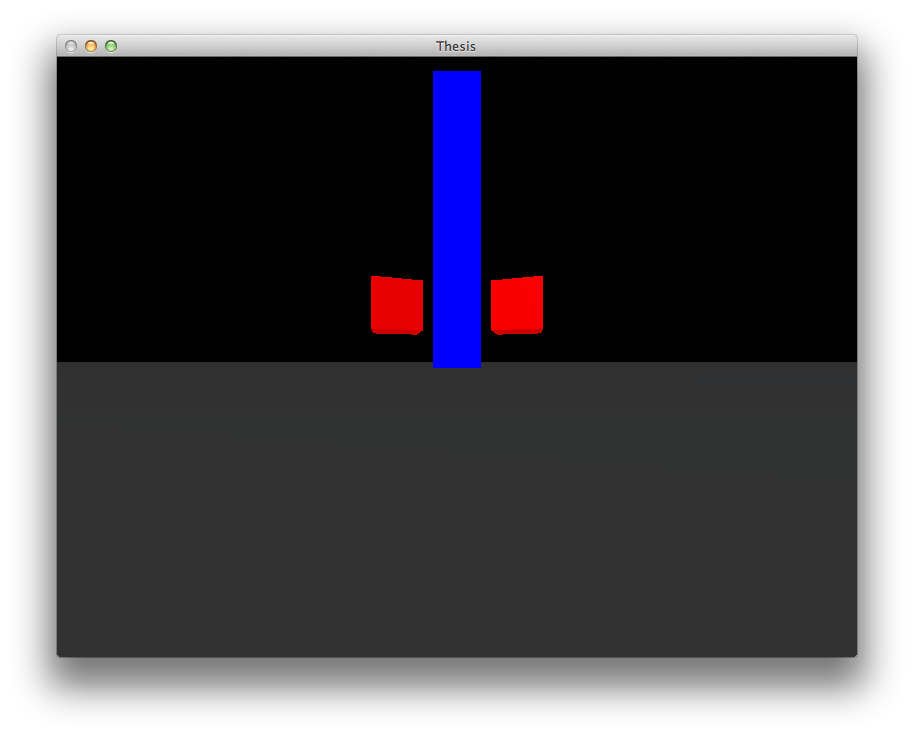
\includegraphics[width=.48\textwidth]{scenario3_rigid}
	  }
	  \subfigure{
	      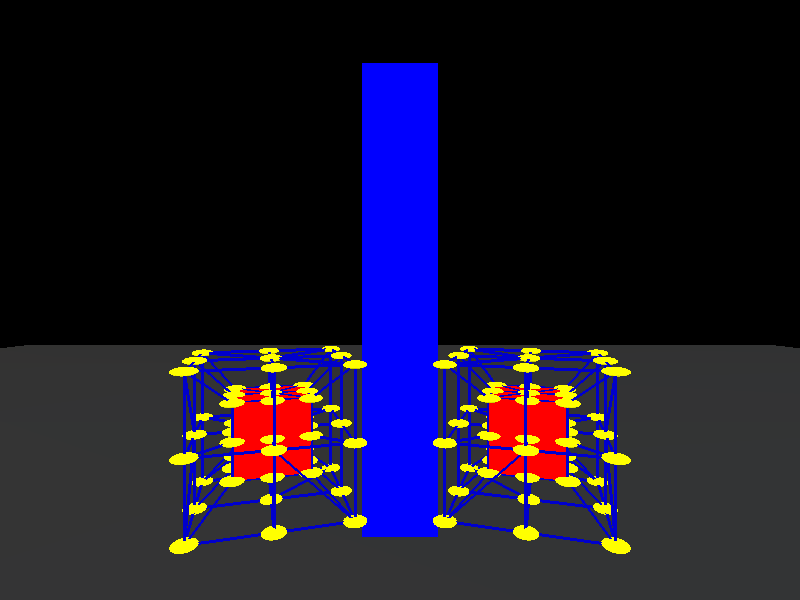
\includegraphics[width=.48\textwidth]{scenario3_combined}
	  }
	\setcounter{subfigure}{0}
	\subfigure[rigid fingers]{
		\begin{tikzpicture}
			\begin{axis}[xlabel=$time$,ylabel=$delta$]
				\addplot [color=red,mark=false,smooth,thick] table[x=time,y=err_x] {data/scenario3_rigid.txt};
				\addplot [color=green,mark=false,smooth,thick] table[x=time,y=err_y] {data/scenario3_rigid.txt};
				\addplot [color=blue,mark=false,smooth,thick] table[x=time,y=err_z] {data/scenario3_rigid.txt};
				\legend{$\Delta x$,$\Delta y$,$\Delta z$}
			\end{axis}
		\end{tikzpicture}
	}
	\subfigure[combined fingers]{
		\begin{tikzpicture}
			\begin{axis}[xlabel=$time$,ylabel=$delta$,legend pos=north west]
				\addplot [color=red,mark=false,smooth,thick] table[x=time,y=err_x] {data/scenario3_combined.txt};
				\addplot [color=green,mark=false,smooth,thick] table[x=time,y=err_y] {data/scenario3_combined.txt};
				\addplot [color=blue,mark=false,smooth,thick] table[x=time,y=err_z] {data/scenario3_combined.txt};
				\legend{$\Delta x$,$\Delta y$,$\Delta z$}
			\end{axis}
		\end{tikzpicture}
	}
	\caption{Evaluation Scenario 3}
\end{figure}

Comparing the rigid fingers to the previous scenario clearly shows how the higher center of mass accelerates the occurrence of the slipping event. The blocks starts to fall sooner and again lands on its side. The combined body simulation on the other hand can handle this scenario just as well as before showing almost no difference. The small jitter\footnote{$Range(\Delta z)=0.81087013$} observed in the previous scenario is a little stronger now as the center of mass has more space to tilt, however it is always realigned by the particles resulting in an almost flat line for $\Delta x$ and $\Delta z$.

\clearpage
\paragraph{Scenario 4}
In the fourth scenario the size of the block has been enlarged so that  it is larger than the surface of the connecting fingers. The soft tissue of the fingers can now no longer surround the complete block but only conforms to the surface.

\begin{figure}[htb]
	\setcounter{subfigure}{0}
	\centering
	  \subfigure{
	      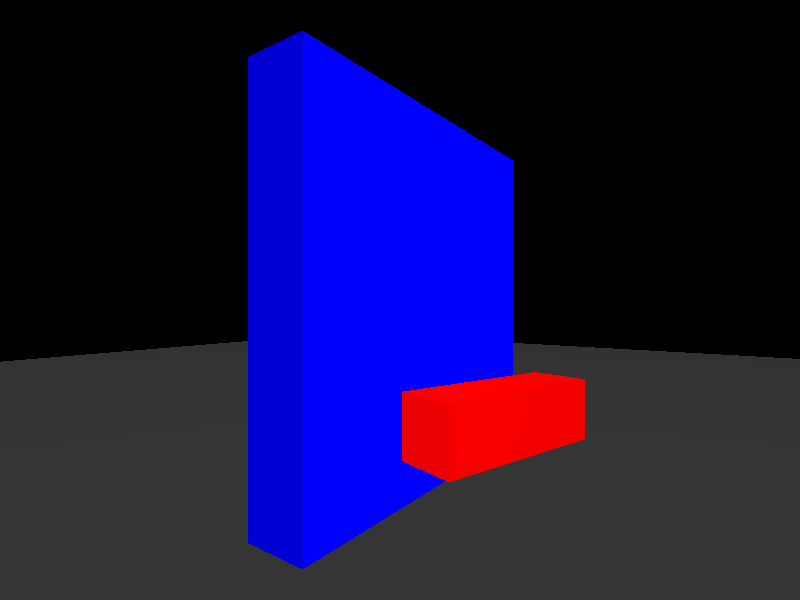
\includegraphics[width=.48\textwidth]{scenario4_rigid}
	  }
	  \subfigure{
	      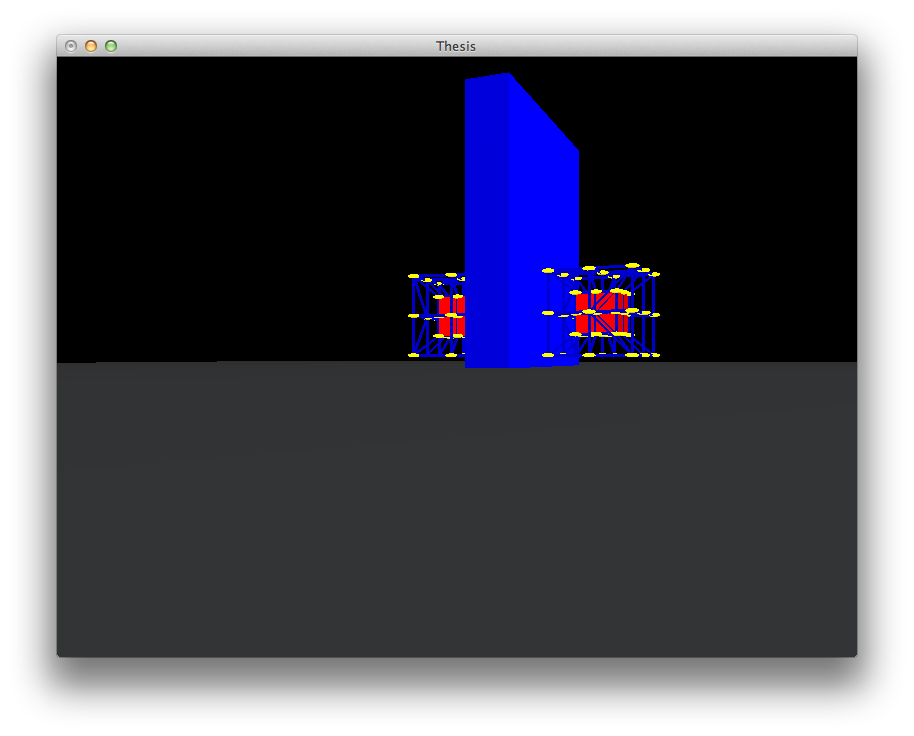
\includegraphics[width=.48\textwidth]{scenario4_combined}
	  }
	\setcounter{subfigure}{0}
	\subfigure[rigid fingers]{
		\begin{tikzpicture}
			\begin{axis}[xlabel=$time$,ylabel=$delta$,legend pos=north west]
				\addplot [color=red,mark=false,smooth,thick] table[x=time,y=err_x] {data/scenario4_rigid.txt};
				\addplot [color=green,mark=false,smooth,thick] table[x=time,y=err_y] {data/scenario4_rigid.txt};
				\addplot [color=blue,mark=false,smooth,thick] table[x=time,y=err_z] {data/scenario4_rigid.txt};
				\legend{$\Delta x$,$\Delta y$,$\Delta z$}
			\end{axis}
		\end{tikzpicture}
	}
	\subfigure[combined fingers]{
		\begin{tikzpicture}
			\begin{axis}[xlabel=$time$,ylabel=$delta$,legend pos=north west]
				\addplot [color=red,mark=false,smooth,thick] table[x=time,y=err_x] {data/scenario4_combined.txt};
				\addplot [color=green,mark=false,smooth,thick] table[x=time,y=err_y] {data/scenario4_combined.txt};
				\addplot [color=blue,mark=false,smooth,thick] table[x=time,y=err_z] {data/scenario4_combined.txt};
				\legend{$\Delta x$,$\Delta y$,$\Delta z$}
			\end{axis}
		\end{tikzpicture}
	}
	\caption{Evaluation Scenario 4}
\end{figure}

The results for this scenario are interesting. The rigid body simulation performs surprisingly well. The reason for this behavior is the fact that the block now can now no longer be pushed out of the two fingers. The lift off is delayed because the block is rotating around the very small connected edges. The combined simulation continues to perform very well. Despite some variance in both $\Delta x$ and $\Delta y$ caused by the larger leverage force of the block the simulation is slowly accelerating upwards.
